\chapter{RPG Notation Style}\label{chap:notation}

This chapter presents some conventions on notation that we use at the Robotics and Perception Group.
Try to stick to those conventions since a unique style makes it easier to review the report.

\section{Variable styles in \LaTeX}

Use lowercase and bold letters for vectors, e.g. $\textbf{x}$, uppercase and bold letters for matrices, e.g. $\textbf{R}$, and lowercase letters with normal weight for scalars, e.g. $s$.

\section{Coordinate Systems and Rotations}

We use the notation introduced by Prof. Glocker in the course ``Mechanik 3'' at ETHZ to express coordinate frames, rotations and vectors.
Refer to Chapter~5 ``Kinematik'' in the lecture script for more details \footnote{\url{http://mitschriften.amiv.ethz.ch/main.php?page=3&scrid=1&pid=87&eid=1}}.
Figure \ref{fig:notation} gives an overview of how coordinate transformations and vectors are specified.
Observe that the coordinate system in which a vector is expressed is always written as index before the variable, e.g. $_B\mathbf{t}_{AB}$ is the vector from $A$ to $B$ expressed the coordinate system $B$.
For the ease of reading, the index for the origin coordinate frame can be omitted: $_O\mathbf{t}_k := \mathbf{t}_k$.

\begin{figure}[H]
     \centering
     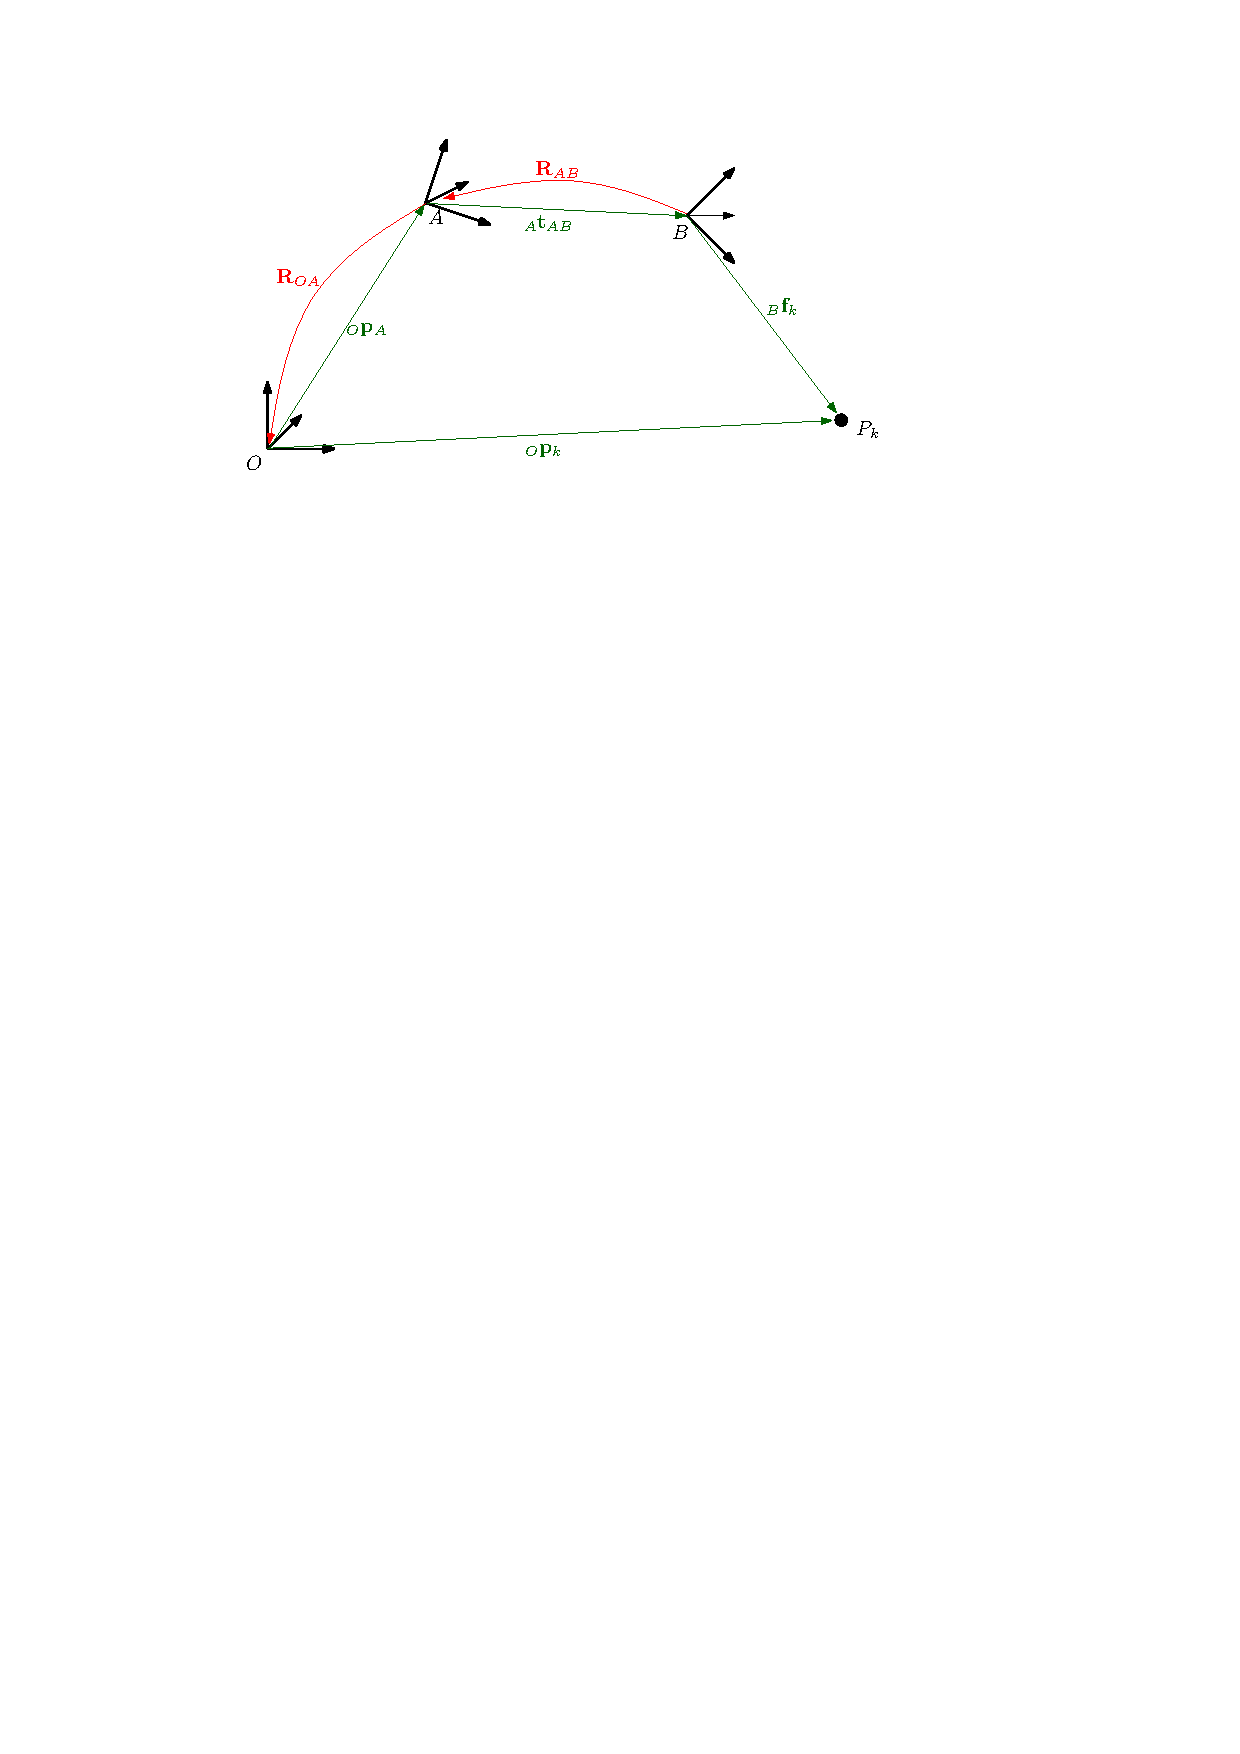
\includegraphics[scale=0.8]{img/notation}
     \caption{Notation overview.}
     \label{fig:notation}
\end{figure}
  
$A$ and $B$ are two adjacent coordinate frames and $O$ is the frame of origin.
$\mathbf{R}_{AB}$ describes the coordinate transformation from frame $B$ to frame $A$, thus it holds that 
	\[
		\begin{aligned}
			_O\mathbf{t}_k  &= \mathbf{R}_{OB} \ _B\mathbf{f}_k, \\
			\mathbf{R}_{OB} &= \mathbf{R}_{OA} \ \mathbf{R}_{AB}.
	  \end{aligned} 
	\]

\section{Measured, estimated and target values}

For controllers and estimators please specify the variables as follows in the report:

	\[
		\begin{aligned}
			\text{true value:} \quad & \mathbf{x} \\
			\text{estimated value:} \quad & \hat{\mathbf{x}} \\
			\text{measured value:} \quad & \tilde{\mathbf{x}} \\
			\text{desired value:} \quad & \mathbf{x}_\text{des} \\
      \text{error value:} \quad & \mathbf{x}_\text{e} \\
      \text{equilibrium value:} \quad & \mathbf{x}^* \\
		\end{aligned}
	\]
